\documentclass[11pt]{article}
\usepackage[review]{acl}
\usepackage{times}
\usepackage{latexsym}
\usepackage[T1]{fontenc}
\usepackage[utf8]{inputenc}
\usepackage{microtype}
\usepackage{amsmath,amssymb}
\usepackage{booktabs}
\usepackage{graphicx}
\usepackage{xcolor}
\setcounter{dbltopnumber}{4}
\renewcommand{\dbltopfraction}{0.93}
\makeatletter
\setlength{\@fptop}{0pt}
\setlength{\@fpsep}{12pt}
\setlength{\@dblfptop}{0pt}
\setlength{\@dblfpsep}{12pt}
\makeatother
\title{Contextual Cartridges: Query-Guided Test-Time Learning\\with Selective Self-Distillation}
\author{Anonymous working draft}
\begin{document}
\maketitle
\begin{abstract}
Compact KV memories offer an alternative to repeatedly reading long documents, but a generic study distribution may spread capacity across irrelevant topics or inadequately supervise the relations needed by an arriving query. We study Contextual Cartridges, which combines answer-guided query-specific synthetic data with conservative selective self-distillation. The latter uses checkpoint-wise leave-one-out gradient alignment to nominate conflicting teacher trajectories and matched deletion refits to test their removal. All updates remain confined to native KV memory. A completed, count-matched synthetic-data audit covers 1,000 BABILong requests and 26,451 exercises per method. It shows reduced zero-support source contexts and increased support-fact coverage and joint exposure. These are data-construction measurements, not answer-accuracy results. The downstream factorial evaluation and cross-model cache curves are explicitly pending in this working draft.
\end{abstract}

\section{Introduction}
Learning a compact document memory can reduce the context retained at inference time. Cartridges train native KV tensors using synthetic conversations and context distillation \citep{eyuboglu2025cartridges}. Their document-level study distribution is designed for future queries. When a query is already available, the study budget can instead concentrate on its relevant facts and relations.

We study two risks of a generic distribution: \emph{dilution}, in which unrelated material consumes study capacity, and \emph{fragmentation}, in which locally covered facts do not provide sufficient joint supervision for the current query. A separate risk concerns supervision: unconditional imitation can absorb conflicting teacher trajectories. We refer to this supervision-design limitation as the \emph{oracle trap}, without assuming any mathematical teacher-performance ceiling.

Contextual Cartridges addresses these risks through two mechanisms. Answer-guided question construction makes query-related conclusions the targets of synthetic practice. Conservative selective SD uses gradient evidence and actual refits to remove trajectories that harm the retained learning objective. The method preserves the frozen backbone and native KV inference interface. Its accuracy benefits remain a hypothesis until the pending paired evaluations are complete.

\section{Method}
\label{sec:method}

Contextual Cartridges adapts a compact native KV memory to a known document--query pair. Given document $D=(C_1,\ldots,C_N)$ and query $q$, we freeze the language model $p_\theta$ and optimize only the request-specific memory $Z=(K_{\mathrm{cart}},V_{\mathrm{cart}})$. We retain the KV parameterization and context-distillation foundation of Cartridges \citep{eyuboglu2025cartridges}. Our two techniques change the study-task distribution and which distillation trajectories are retained. The final answer is generated from $(Z^*,q)$ without appending the source document.

\subsection{Answer-Guided Query-Specific Data}

\paragraph{Why condition self-study on the query?}
Generic study tasks distribute a fixed memory and optimization budget across topics that may not serve the current request (\emph{dilution}). Training on local facts separately may also undersupervise the particular cross-source relation needed by that request (\emph{fragmentation}). These are limitations of a task distribution for a known query, not claims that the original method lacks structural prompts or cannot perform global reasoning.

\paragraph{Source selection and answer-first construction.}
A lightweight decision model or cached relevance scores, supplemented with lexical, entity, and neighboring-source recall, selects a small collection of source groups $E_i\subseteq D$. A group may contain a single chunk or complementary chunks in original order. The frozen generator first extracts a query-relevant conclusion $a_i$, then constructs a closed-book question $s_i$ targeting that conclusion:
\begin{align}
P(E,a,s\mid D,q)={}&P(E\mid D,q)\nonumber\\
&\cdot P_\theta(a\mid E,q)P_\theta(s\mid E,q,a).
\end{align}
The two semantic steps can be emitted sequentially in one generation call. The generator may skip a group that yields no useful conclusion. We save $\mathcal S_q=\{(s_i,a_i,E_i)\}_{i=1}^M$ with source identifiers. Routine empty-item and duplicate checks do not serve as a semantic verifier.

This construction allocates study examples to the current query, while a conclusion drawn from complementary sources provides an opportunity to train their relationship. Neither a source citation nor multiple source chunks proves that a generated answer is correct or requires all of those chunks. We therefore evaluate coverage and joint exposure separately from downstream accuracy.

\paragraph{Frozen dataset convention.}
The BABILong comparison reuses two completed synthetic JSON releases. Its query-specific source groups use cached Decision API single-source scores and deterministic entity/bridge expansion. The cache-curve runner instead uses Qwen3-Reranker-0.6B for candidate ranking. These adapters share the answer-first principle but are not identical retrieval implementations. No synthetic data is regenerated for the figures in this paper.

\subsection{Native KV Self-Distillation}

Each trajectory provides a question $s_i$, a source context $E_i$, and a fixed response sequence $y_i$. At the same answer prefix, the teacher and student distributions are
\begin{align}
p_T^{i,t}&=p_\theta(\cdot\mid E_i,s_i,y_{i,<t}),\\
p_S^{i,t}(Z)&=p_{\theta,Z}(\cdot\mid s_i,y_{i,<t}).
\end{align}
The conceptual objective matches teacher-to-student KL. The implementation retains the upstream sparse soft-target cross-entropy over stored teacher entries $\Omega_i$:
\begin{equation}
\mathcal L_i(Z)=-\frac{1}{|\Omega_i|}\sum_{(t,v)\in\Omega_i}
\operatorname{sg}[p_T^{i,t}(v)]\log p_S^{i,t}(v;Z).
\end{equation}
Student log probabilities use the full vocabulary; retained teacher probabilities are not renormalized. Full-distribution cross-entropy and KL have the same student gradient, but the stored top-$k$ target is still an approximation. All gradients update native KV only; the backbone and teacher targets remain fixed.

For BABILong, the saved synthetic assistant answer is the trajectory $y_i$ on which teacher soft targets are computed. The answer-first output is therefore not discarded after question construction, nor treated as a verified hard-label target. The three-dataset runner generates source-conditioned teacher responses and reuses them across cache capacities. Initialization follows the upstream KV initializer, including its frozen prefix position.

\subsection{Conservative TracIn-Guided Selective SD}

\paragraph{Motivation and fixed training budget.}
Unconditionally learning every teacher trajectory can introduce conflicting supervision into shared memory. We call this the \emph{oracle trap}; it is not a theorem bounding the student by teacher accuracy. Our selector defaults to retaining a trajectory and requires both consistent gradient opposition and an actual deletion benefit before removing it.

Let $R_0$ be the complete usable trajectory set. For any retained subset $R$, define
\begin{equation}
Z_R^{(b)}=\operatorname{SD}_T(Z_0;R,\pi_b),\quad b\in\{1,2\},
\end{equation}
where $\pi_b$ are two predetermined training orders. Every fit starts from the same $Z_0$ with a fresh Adam state, the same learning rate, and $T$ optimizer updates. The primary full-data ordinary-SD pilot determines $T$; in BABILong the query-agnostic pilot sets $T$ for both dataset arms. Matching final update counts does not match total selection compute.

\paragraph{Checkpoint-wise leave-one-out nomination.}
Inspired by TracIn \citep{pruthi2020tracin}, we compute KV gradients at the shared initialization and both current fitted endpoints, $\mathcal C_R=\{Z_0,Z_R^{(1)},Z_R^{(2)}\}$:
\begin{align}
g_{i,c}&=\nabla_Z\mathcal L_i(Z_c),\\
\bar g_{-i,c}&=\frac{1}{|R|-1}\sum_{j\in R\setminus\{i\}}g_{j,c},\\
u_{i,c}&=\bar g_{-i,c}^{\top}g_{i,c}.
\end{align}
Excluding the candidate prevents self-influence from producing a positive score by construction. A negative dot product predicts an increase in peers' average loss under a small SGD step. Because actual training uses Adam and multiple updates, this is a nomination proxy, not an exact effect or a truth score.

We nominate $i$ only if $u_{i,c}<0$ at every checkpoint. Nonnegative scores, disagreement, or insufficient peers retain the trajectory. Candidates are tried in ascending order of their largest checkpoint cosine, prioritizing consistent opposition. Unlike the original TracIn sum, a large gradient at one checkpoint cannot overrule another checkpoint's veto.

\paragraph{Confirm deletion by matched refits.}
For a nominee $i$, let $A=R\setminus\{i\}$ and retrain $Z_A^{(1)}$ and $Z_A^{(2)}$. For every survivor $j\in A$ and both orders, require
\begin{align}
\mathcal L_j(Z_A^{(b)})&\leq\mathcal L_j(Z_R^{(b)})+\epsilon_{j,R}^{(b)},\\
\mathcal L_j(Z_A^{(b)})&\leq\mathcal L_j(Z_{R_0}^{(b)})+\epsilon_{j,0}^{(b)},
\end{align}
where each tolerance is $10^{-6}+10^{-5}|\mathcal L_{\mathrm{reference}}|$. Survivor mean loss must also improve over the current fit by more than the mean tolerance under each order. The original-pilot guard limits cumulative tolerance drift. Any failed condition rejects deletion.

After an accepted deletion, we replace $R$ with $A$, update both fits, and recompute nomination scores. Selection stops when no deletion passes or one trajectory remains. We return the fixed primary-order fit, never a seed selected by benchmark answers. With no confirmed deletion, the exact already-trained ordinary-SD checkpoint is returned. Selection uncertainty does not cause abstention or an untrained memory.

\paragraph{Scope of protection.}
The guards protect surviving synthetic SD losses, not factual correctness or accuracy on $q$. Correlated teacher errors can survive consensus; deleting a trajectory can still harm a final answer. Extra refits trade computation for stronger evidence about the defined training objective, not a guaranteed accuracy gain. Benchmark labels and held-out probes are not inputs to selection.


\section{Experiments and Completed Data Audit}
\paragraph{Matched synthetic datasets.}
The saved Qwen3-4B-Instruct-2507 datasets contain the same 1,000 BABILong document--query pairs: ten task types and 250 requests at each of 8K, 16K, 32K, and 64K. Each arm contains 26,451 exercises, with counts matched within request and saved split. These figures use the saved query-agnostic Cartridges generation configuration and the query-specific answer-guided configuration; they are not downstream benchmark reproductions of the original paper.

\paragraph{Objective source metrics.}
Let $F_q$ be the post-generation annotated supporting facts for request $q$, and let $F(E_i)$ be those covered by source context $E_i$. We measure the fraction of exercise contexts with no supporting fact, the recall of the union of study contexts, and the fraction co-exposing all facts. Ambiguous source alignment is treated conservatively in the saved lower-bound recall and co-exposure metrics. We first average within a request, then weight requests equally. The multiple-fact analysis uses 352 requests, 88 per document length; it does not require their facts to fall in different original chunks. Six missing query-agnostic recall values are excluded from paired recall only.

\begin{table*}[t]
\centering
\small
\caption{Matched synthetic-data audit: 26,451 exercises per method across 1,000 requests. Means weight requests equally. All-fact co-exposure uses 352 multi-fact requests; recall uses 994 paired requests. These source-coverage proxies do not measure answer correctness or establish necessary multi-hop reasoning.}
\label{tab:synthetic}
\begin{tabular}{lrrrr}
\toprule
Metric & Paired $n$ & Query-agnostic & Query-specific & Difference \\
\midrule
Zero-support contexts (\%) & 1000 & 83.69 & 50.21 & -33.47 \\
Support-fact recall (\%) & 994 & 50.25 & 95.45 & +45.20 \\
All-fact co-exposure (\%) & 352 & 2.48 & 15.15 & +12.67 \\
Evidence characters & 1000 & 7894.13 & 2221.48 & -5672.65 \\
Question words & 1000 & 58.01 & 15.03 & -42.97 \\
\bottomrule
\end{tabular}
\end{table*}


\begin{figure*}[t]
\centering
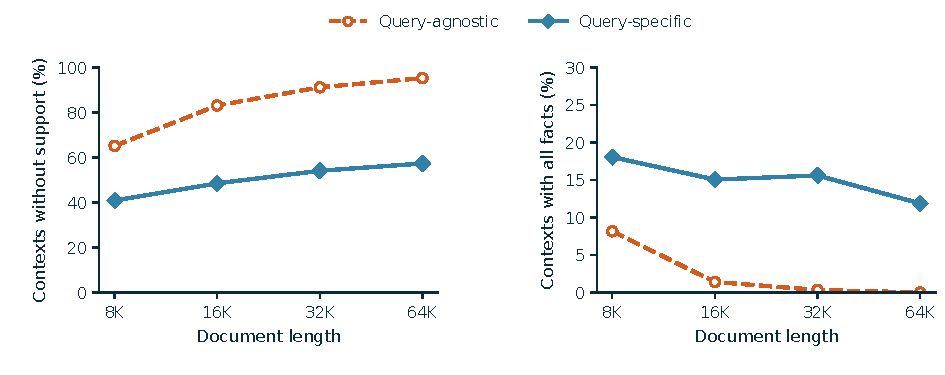
\includegraphics[width=\textwidth]{figures/figure1_dilution_fragmentation.pdf}
\caption{Dilution and joint evidence exposure at four measured document lengths. Left: exercise contexts without any annotated query support (lower is better; 1,000 paired requests). Right: all-fact co-exposure lower bound on 352 multi-fact requests (higher is better). Points are request-macro means. Joint exposure is not a proof of necessary cross-chunk reasoning or correct answers.}
\label{fig:curves}
\end{figure*}

\begin{figure*}[t]
\centering
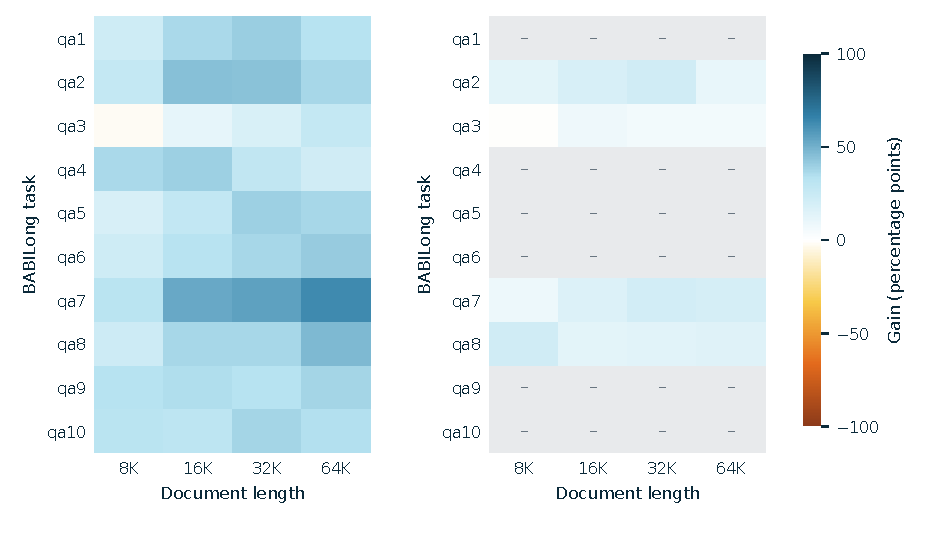
\includegraphics[width=\textwidth]{figures/figure2_task_length.pdf}
\caption{Task--length contrasts. Left: reduction in zero-support context fraction. Right: increase in all-fact co-exposure on eligible multi-fact requests. Positive gains favor query-specific data. Both maps use the same $[-100,100]$ percentage-point scale. Grey cells with dashes have no eligible multi-fact requests; they are not zeros. All task--length groups are retained.}
\label{fig:heatmap}
\vspace{8pt}
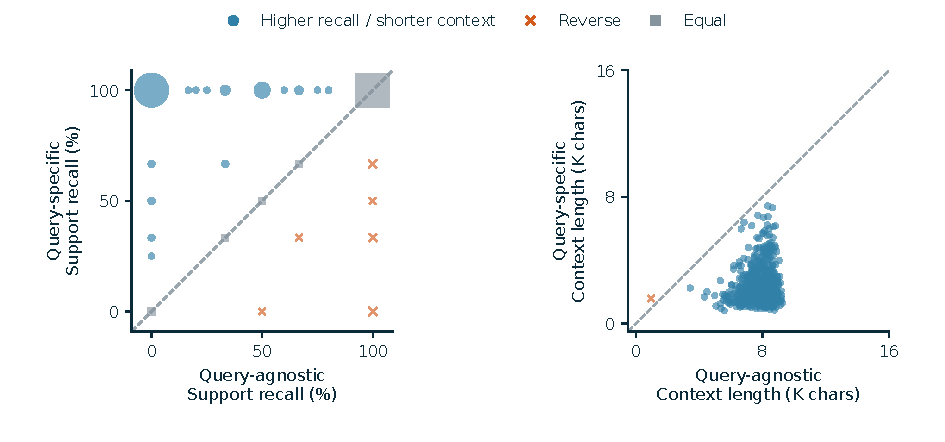
\includegraphics[width=\textwidth]{figures/figure3_paired_coverage_footprint.pdf}
\caption{Paired source coverage and footprint. Left: support-fact recall lower bound on 994 paired requests; identical coordinate pairs are combined with marker area $9+0.65n$ squared points, where $n$ is their multiplicity. Right: source characters per exercise on all 1,000 requests, in thousands. The diagonal is equality. Blue circles indicate higher recall or shorter context; orange crosses indicate the reverse. No jitter or fitted trend is used. Characters are not latency or GPU memory.}
\label{fig:paired}
\end{figure*}

\paragraph{Observed differences.}
Zero-support contexts decrease from 83.69\% to 50.21\%, and paired support recall increases from 50.25\% to 95.45\%. On multi-fact requests, all-fact co-exposure rises from 2.48\% to 15.15\%. Mean source footprint decreases from 7,894 to 2,221 characters per exercise. Figures~\ref{fig:curves}--\ref{fig:paired} retain the length breakdown and paired reverse cases. These measurements establish changes in source coverage and organization, not semantic correctness, necessary multi-hop reasoning, or end-to-end speed.

\paragraph{Pending BABILong factorial evaluation.}
We reserve the full query-agnostic/query-specific $\times$ ordinary/selective SD design. Each completed comparison must use identical requests, model initialization, KV size, and final update count; all additional selection computation is reported separately. Benchmark answers enter only post-generation scoring. In addition to aggregate accuracy, the final evaluation must report corrected and regressed answers. Tables~\ref{tab:babilong-overall} and~\ref{tab:babilong-length} remain empty until their full paired denominators are available.

\begin{table*}[t]
\centering
\small
\setlength{\tabcolsep}{4pt}
\caption{BABILong accuracy over 1,000 requests per backbone. V-SD and S-SD denote ordinary and selective self-distillation. Contextual uses query-specific data and S-SD. $\Delta$ is S-SD minus V-SD on the same query-specific data. All entries are pending (\textemdash); historical configurations are not substituted.}
\label{tab:babilong-overall}
\begin{tabular}{lrrrrrr}
\toprule
Model & ICL & Agn./V-SD & Agn./S-SD & Spec./V-SD & Contextual & $\Delta$ \\
\midrule
Qwen3-4B & \textemdash & \textemdash & \textemdash & \textemdash & \textemdash & \textemdash \\
OLMo-3-7B & \textemdash & \textemdash & \textemdash & \textemdash & \textemdash & \textemdash \\
GPT-OSS-20B & \textemdash & \textemdash & \textemdash & \textemdash & \textemdash & \textemdash \\
\bottomrule
\end{tabular}
\end{table*}

\begin{table*}[t]
\centering
\small
\setlength{\tabcolsep}{4pt}
\caption{BABILong accuracy by document length (250 requests per cell). V-SD and S-SD denote ordinary and selective self-distillation. Contextual uses query-specific data and S-SD. $\Delta$ is S-SD minus V-SD on the same query-specific data. All entries are pending (\textemdash); historical configurations are not substituted.}
\label{tab:babilong-length}
\begin{tabular}{llrrrrrr}
\toprule
Model & Length & ICL & Agn./V-SD & Agn./S-SD & Spec./V-SD & Contextual & $\Delta$ \\
\midrule
Qwen3-4B & 8K & \textemdash & \textemdash & \textemdash & \textemdash & \textemdash & \textemdash \\
Qwen3-4B & 16K & \textemdash & \textemdash & \textemdash & \textemdash & \textemdash & \textemdash \\
Qwen3-4B & 32K & \textemdash & \textemdash & \textemdash & \textemdash & \textemdash & \textemdash \\
Qwen3-4B & 64K & \textemdash & \textemdash & \textemdash & \textemdash & \textemdash & \textemdash \\
OLMo-3-7B & 8K & \textemdash & \textemdash & \textemdash & \textemdash & \textemdash & \textemdash \\
OLMo-3-7B & 16K & \textemdash & \textemdash & \textemdash & \textemdash & \textemdash & \textemdash \\
OLMo-3-7B & 32K & \textemdash & \textemdash & \textemdash & \textemdash & \textemdash & \textemdash \\
OLMo-3-7B & 64K & \textemdash & \textemdash & \textemdash & \textemdash & \textemdash & \textemdash \\
GPT-OSS-20B & 8K & \textemdash & \textemdash & \textemdash & \textemdash & \textemdash & \textemdash \\
GPT-OSS-20B & 16K & \textemdash & \textemdash & \textemdash & \textemdash & \textemdash & \textemdash \\
GPT-OSS-20B & 32K & \textemdash & \textemdash & \textemdash & \textemdash & \textemdash & \textemdash \\
GPT-OSS-20B & 64K & \textemdash & \textemdash & \textemdash & \textemdash & \textemdash & \textemdash \\
\bottomrule
\end{tabular}
\end{table*}


\paragraph{Pending cache--performance evaluation.}
We reserve Qwen3-4B, OLMo-3-7B, and GPT-OSS-20B across LongHealth, MTOB (KE), and QASPER, with 512/1,024/2,048/4,096 KV positions. The respective metrics are accuracy, corpus chrF, and mean gold-answer log-perplexity, as in the Cartridges benchmark comparison. Figure~\ref{fig:cache} is an explicit placeholder. Each curve requires the same paired cases at all capacities. Published baselines must retain their original backbone and protocol and cannot be transferred to another model's panel.

\begin{figure*}[t]
\centering
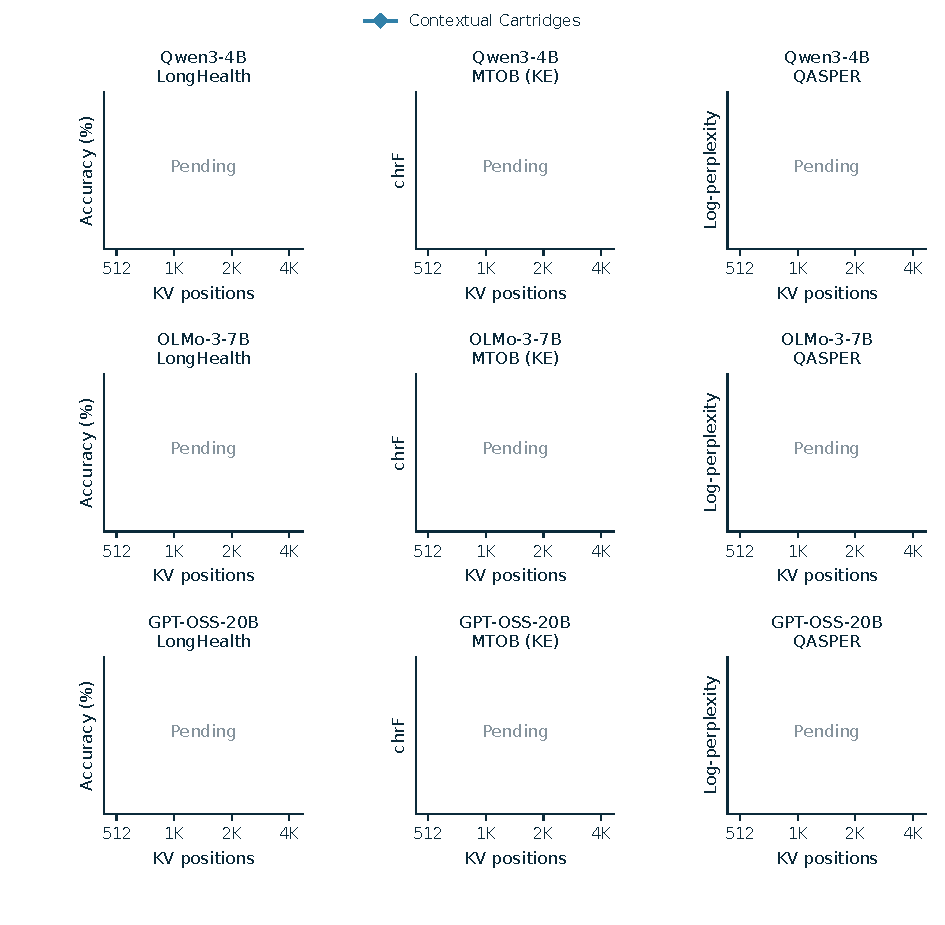
\includegraphics[width=\textwidth]{figures/figure4_cache_grid_pending.pdf}
\caption{Pending cache--performance matrix: three backbones, three datasets, and four capacities. No measured points are populated in this draft. Accuracy and chrF are higher-is-better; log-perplexity is lower-is-better. KV positions are a logical capacity, not an equal byte budget across architectures. The panels reserve experiments and do not imply that all backbones have completed or are currently scheduled.}
\label{fig:cache}
\end{figure*}

\clearpage
\section{Limitations}
Source recall and co-exposure do not certify a generated answer or establish that a question requires every source. Correlated teacher errors can remain mutually consistent. The selective guard controls synthetic SD losses rather than benchmark correctness, and raw gradient alignment is only a local proxy for actual Adam dynamics. Confirmatory refits add substantial online cost. Per-query preparation is not amortized across arbitrary future queries as in the original document-level setting. The current paper contains completed data audits and pending downstream evaluations; it does not claim that the method already surpasses ordinary SD, the teacher, or full-context inference.

\section*{Reproducibility}
The accompanying package includes the immutable per-request figure snapshot, CSVs, explicit-null result templates, plotting/table scripts, the current selector snapshot, and export hashes. Figures are vector PDFs with embedded fonts, plus editable SVGs and 400-DPI PNGs. The preparation workflow follows scientific-visualization \citep{kassis2026skills}; this is a software acknowledgment, not an empirical validation.

\begin{thebibliography}{3}
\bibitem[Eyuboglu et~al.(2025)]{eyuboglu2025cartridges}
Sabri Eyuboglu, Ryan Ehrlich, Simran Arora, Neel Guha, Dylan Zinsley, Emily Liu, Will Tennien, Atri Rudra, James Zou, Azalia Mirhoseini, and Christopher R\'{e}. 2025.
\newblock \href{https://arxiv.org/abs/2506.06266}{Cartridges: Lightweight and general-purpose long context representations via self-study}.
\newblock arXiv:2506.06266.
\bibitem[Pruthi et~al.(2020)]{pruthi2020tracin}
Garima Pruthi, Frederick Liu, Satyen Kale, and Mukund Sundararajan. 2020.
\newblock \href{https://proceedings.neurips.cc/paper/2020/hash/e6385d39ec9394f2f3a354d9d2b88eec-Abstract.html}{Estimating training data influence by tracing gradient descent}.
\newblock In \emph{Advances in Neural Information Processing Systems 33}.
\bibitem[Kassis et~al.(2026)]{kassis2026skills}
Timothy Kassis, Vinayak Agarwal, Yuhuan He, Darshil Patel, and Aubrey~M. Brueckner. 2026.
\newblock \href{https://doi.org/10.48550/arXiv.2609.00065}{Scientific Agent Skills: A library of procedural knowledge for research agents}.
\newblock arXiv:2609.00065.
\end{thebibliography}
\end{document}
